\documentclass{article} % For LaTeX2e
\usepackage{nips13submit_e,times}
\usepackage{hyperref}
\usepackage{url}
\usepackage{graphicx}
\usepackage{subcaption}
\usepackage{afterpage}
%\documentstyle[nips13submit_09,times,art10]{article} % For LaTeX 2.09


\title{Predicting Game Play Direction in Football Videos}


\author{
Amit Bawaskar\\
School of EECS\\
Oregon State University\\
\texttt{bawaskar@onid.orst.edu} \\
\And
Michael Lam \\
School of EECS\\
Oregon State University \\
\texttt{lamm@onid.orst.edu} \\
}

% The \author macro works with any number of authors. There are two commands
% used to separate the names and addresses of multiple authors: \And and \AND.
%
% Using \And between authors leaves it to \LaTeX{} to determine where to break
% the lines. Using \AND forces a linebreak at that point. So, if \LaTeX{}
% puts 3 of 4 authors names on the first line, and the last on the second
% line, try using \AND instead of \And before the third author name.

\newcommand{\fix}{\marginpar{FIX}}
\newcommand{\new}{\marginpar{NEW}}

\nipsfinalcopy % Uncomment for camera-ready version

\begin{document}


\maketitle

\begin{abstract}
The aim of this project is to make a machine learning system which will detect the direction in which the offensive team is playing in football videos. This information is necessary when we have to make automated computer vision systems which will provide us with analysis of the footabll games for coaching purposes. To develop such a system, we have used the KLT Tracking system to track seemingly interesting points in the videos, and then use machine learning algorithms of Decision Tree and Decision Stump with Boosting to identify which player tracks are important in making the decision for the direction of the offensive play. 
%The abstract paragraph should be indented 1/2~inch (3~picas) on both left and
%right-hand margins. Use 10~point type, with a vertical spacing of 11~points.
%The word \textbf{Abstract} must be centered, bold, and in point size 12. Two
%line spaces precede the abstract. The abstract must be limited to one
%paragraph.
\end{abstract}

\section{Introduction}
%\textbf{Clearly state the problem. Motivate the problem.}

To come up with good and effective solutions for football coaching software, we require to track players, look for prominently used strategies by different teams, etc. In general we need to find all those properties of a football video that the coach can use to better train his own team, given a set of videos of the opposition team. To do so, in the absence of such a coaching software, the coach or his team of assistants have to look at numerous plays of the team and decipher the playing strategy of the teams. Even after the coach is done doing this, he now has to send out a great deal of documentation to the players so that they know their roles in the game. This leads to a lot of time spent in auxiliary work which could have been automated. 

The aim of this project is to help develop a part of such a coaching software. This project will aim at recognizing the direction of the offensive play given a video. This analysis can then be used to make comments about the team that is on offense, the orientation of the players on the offensive team and the player movements in both the teams. It will serve as a major step in developing the coaching software as many other elements of the coaching software are dependent on it.

\section{Methodology}
%\textbf{Motivate the method and explain why chose it.}

\afterpage{
\begin{figure}
\centering
 \begin{subfigure}{.24\textwidth}
  \centering
  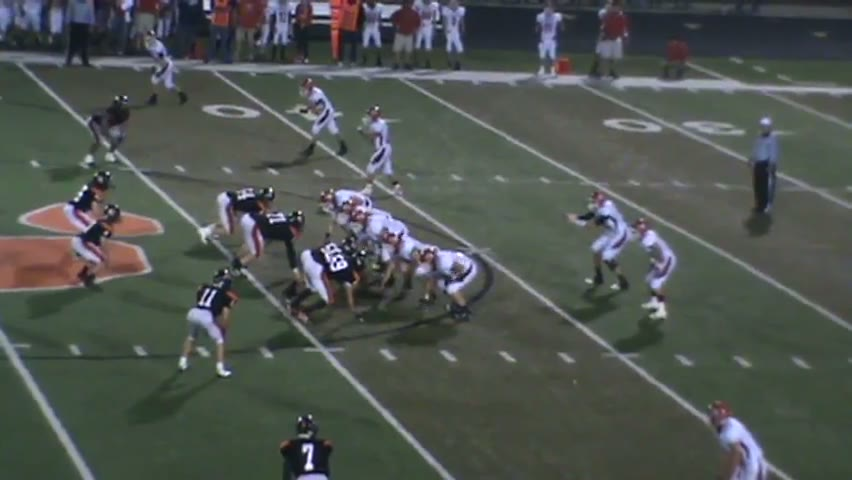
\includegraphics[width=1\linewidth]{img/football_frame1.jpg}
 \end{subfigure}\hspace{.5em}%
 \begin{subfigure}{.24\textwidth}
  \centering
  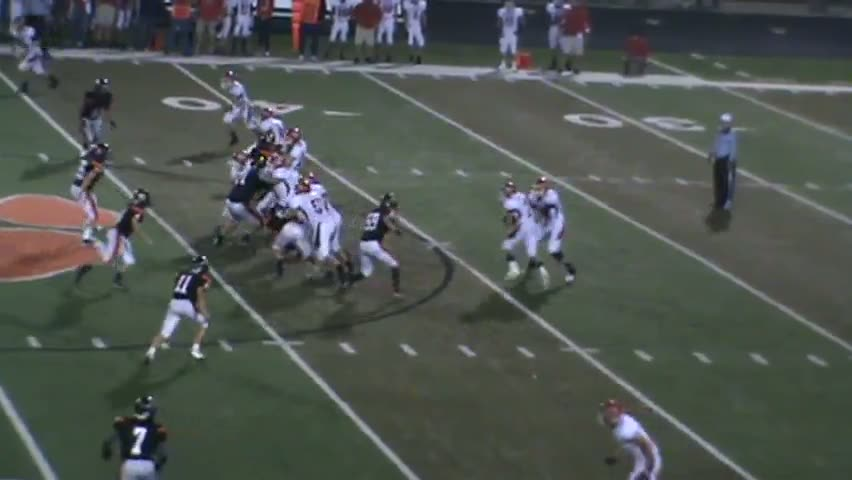
\includegraphics[width=1\linewidth]{img/football_frame2.jpg}
 \end{subfigure}\hspace{.5em}%
 \begin{subfigure}{.24\textwidth}
  \centering
  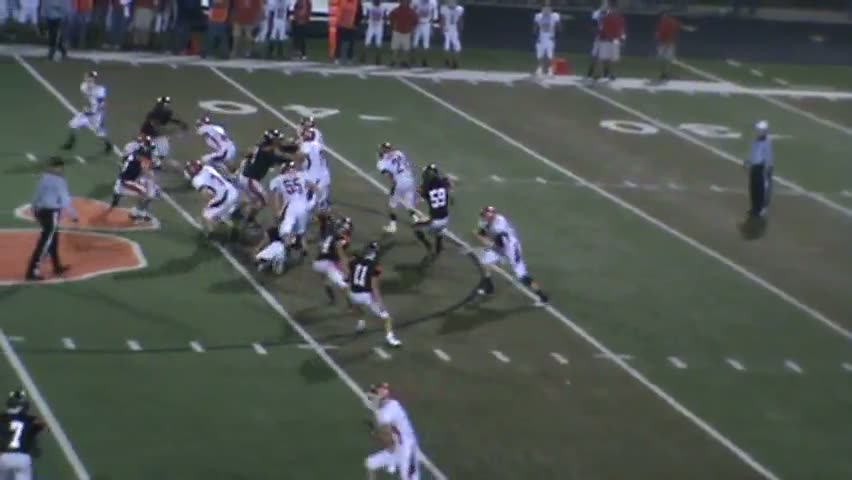
\includegraphics[width=1\linewidth]{img/football_frame3.jpg}
 \end{subfigure}\hspace{.5em}%
 \begin{subfigure}{.24\textwidth}
  \centering
  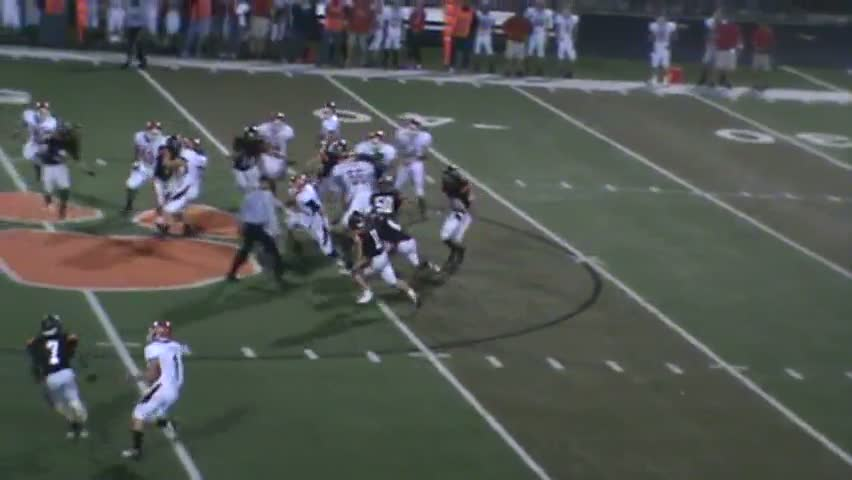
\includegraphics[width=1\linewidth]{img/football_frame4.jpg}
 \end{subfigure}
\caption{An example sequence of a particular football play video footage. Note the wide receiver (bottommost player in white) dashes off to the left. The goal is to classify this video as ``left'' by tracking the wide receiver.}
\label{fig:football}
\end{figure}
}

In order to recognize the direction of offense we need to know some domain knowledge about football. We will provide with a brief overview of the domain knowledge that we require for this project. Usually when the two teams line up for a play in the game of football, we have two players known as ``Wide Receivers'' standing at the ends of the field along the line of scrimmage. The line of scrimmage is the line that separates the two teams at the moment of snap. The moment of snap is the time at which the players start to play the game for each play. 

These two wide receivers are instrumental in the detection of the direction of the play as they run fast down the field in the direction of offense from the moment of snap and can be used to determine the direction of the play. If we are able to get good, long tracks on these players, and if we are able to tell that these tracks belong to the wide receivers, we can find the direction of those tracks and ultimately determine the offensive direction of play. Figure \ref{fig:football} shows an example of video footage where the wide receiver runs fast down the field in the direction of offense, which is to the left of the video frame.

We decided to use KLT tracks [1,2,3] to do the video tracking on different points in the video. The KLT tracking method selects points that have a high gradient with respect to its neighbors. This makes it select ``interesting'' points such as corners in the video frame. We want to use these interesting points and specify which of these points correspond to the wide receiver on the field. Using KLT tracks, we can get the length of the track easily by simple geometric computation on the track features. Also, we can get the distance of the track from the bottom edge of the frame. Figure \ref{fig:klt} visualizes these KLT tracks.

We use KLT tracks to generate a dataset for the videos with the following features:

\begin{enumerate}
	\item Track Number
	\item Starting Point Co-ordinates of the track
	\item Ending Point Co-ordinates of the track
	\item Normalized length of the track.
	\item Normalized distance of the track from the bottom edge of the figure.
	\item Direction of the track.
\end{enumerate}

After getting such a dataset from the KLT tracks, we have to find out a way to determine which of these tracks belong to the wide receiver. We can now use the domain knowledge to determine where to look for the receivers. They will be at the near end and the far end of the field. Also, since they run fast, they will have longer tracks as compared to anyone else on the field. Hence, we have to look for long tracks on both the ends of the field.

We can plot a sample dataset as shown in the following image.

IMAGE!

Here the $y$-direction represents the length of the track while the $x$ direction represents the closeness to the bottom edge of the field. If $x = 1$, then the track is nearest to the bottom. If $x = 0$ then it is farthest from the bottom.

Now, we have to find a region in this plot where the receiver tracks will be. Using the domain knowledge and the inspection of various videos, we come to know that the receiver tracks will more often than not be in the highlighted part in the figure. But, this region will change from video to video as the orientation of the videos, the resolution quality and even plays will be different in different situations. Here is where we use the machine learning algorithms to determine the rectangle to be considered for determining the direction of play. 

We then use a machine learning algorithm to identify the best rectangle which will denote the direction of play. We predict the direction of play by considering a majority vote of all the tracks that fall within the rectangle. If the majority are moving in left direction we say that the direction of the play is left.

\section{Features}
%\textbf{Explain how we formulated features.}

The features that we have considered here are as follows:

\textbf{a. Length of the track.}

We know from the domain knowledge that the wide player will be the one who will make a big rush down field so that we will get good, continuous and long tracks on him. Also, the other players, like free safety, quarter back or the guard players will not move much in the first one and a half second and will have relatively smaller tracks. So, we wish to select those tracks that have a high length as feature.

\textbf{b. Distance from the edge of the field.}

As mentioned before we know that the wide players will be on the near side of the field. The orientation of the play recording is always such that the wide player that we want to track will always be on the bottom most part of the frame. So, we have selected the distance from the edge of the field as our next feature. 

\textbf{c. Track direction with respect to the field.}

This information is vital, since one player will have multiple tracks in one and a half second which will all be close by and going along the same direction. So, if we include the information of the direction of the track (left or right) we will be able to make the differentiation between the noisy tracks and actual wide player tracks better. Thus, the reason for selecting this as a feature.

\begin{figure}
\centering
 \begin{subfigure}{.32\textwidth}
  \centering
  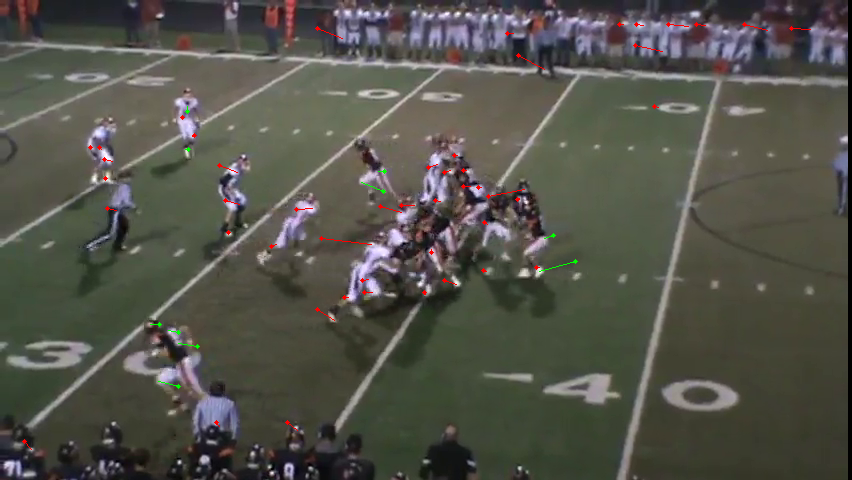
\includegraphics[width=1\linewidth]{img/127.png}
 \end{subfigure}\hspace{.5em}%
 \begin{subfigure}{.32\textwidth}
  \centering
  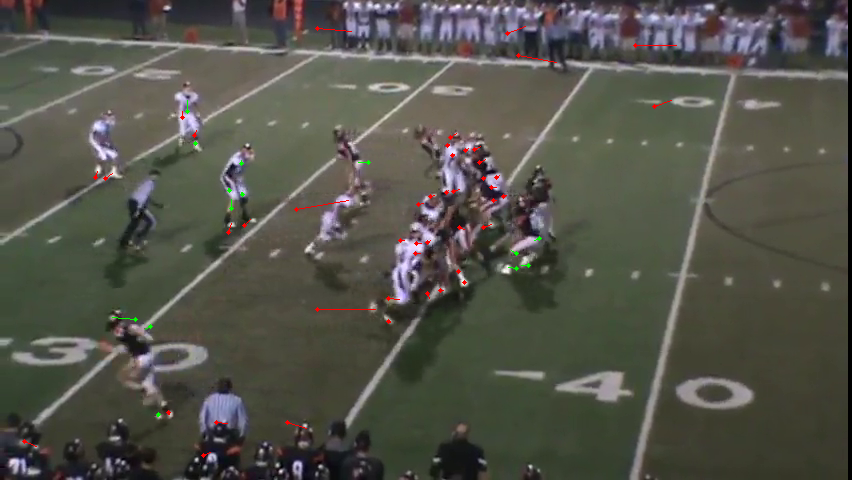
\includegraphics[width=1\linewidth]{img/132.png}
 \end{subfigure}\hspace{.5em}%
 \begin{subfigure}{.32\textwidth}
  \centering
  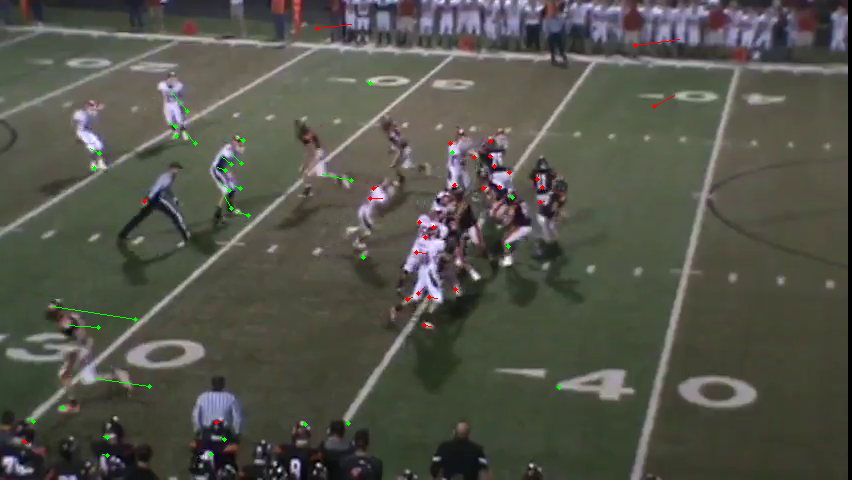
\includegraphics[width=1\linewidth]{img/137.png}
 \end{subfigure}\hspace{.5em}%
\caption{Another example sequence of a particular football play shown with KLT tracks extracted. Green tracks denote left direction and red tracks denote right direction. Faster moving objects have longer tracks. Using domain knowledge, we can make a good guess for which tracks in a video belong to the wide receiver. Note the wide receiver (bottommost player in black) dashes off to the left. The green KLT tracks on this player get longer and are near to the edge of the field.}
\label{fig:klt}
\end{figure}

In short, we want to track those points that have a high length and are closer to the edge of the field, moving in one direction so that we can say that the tracked point is a wide receiver. Again, figure \ref{fig:klt} summarizes these features' relevance.

\section{Learning}
%\textbf{Justify learning algorithms.}

Recall that the goal is to learn the best rectangle in the plot where the $y$-direction represents the length of the track while the $x$ direction represents the closeness to the bottom edge of the field. A majority vote of track directions in this rectangle will denote the direction of play.

Our unique strategy is to use many different random rectangles as features for our learning algorithm and learn a linear combination of those features. First we construct many different rectangles with random sizes and positions in the plot. These rectangles are fixed across every video. For each video, we count the number of left and right tracks falling in each rectangle and produce a measure of ``leftness'' and ``rightness'' for that rectangle. Specifically, for a particular rectangle, we add up all left track counts falling in that rectangle, subtract all right track counts and normalize by the number of tracks; this produces a ``net normalized direction count.''

In the end, we use 60 different features (rectangles) for each video to submit to our learning algorithms. These 60 features are ``predictions'' of 60 different rectangles. These 60 features will be our machine learning features to input into a learning algorithm. Since each video is also manually annotated as left or right offensive direction, we can use a supervised machine learning algorithm to learn a hypothesis that predicts the offensive direction given a video.

Our strategy naturally lends to using boosting since we want to learn a linear combination of weak classifiers. Our weak classifiers can be decision stumps operating on one feature, which is some rectangle in the plot. Each feature would be given a weight for the final prediction. We decided to use AdaBoost [4] as our meta-learning algorithm with decision stumps as the base learner.

We also decided to use decision trees [5] to compare our results with AdaBoost since it is tree-based. We used the C4.5 algorithm for generating the decision tree based on information gain. Since our features are continuous, we also threshold each feature and select the threshold that maximizes the information gain, before selecting the maximum information gain from all the features. Note that the decision stump is simply a one-level version of the decision tree used in the AdaBoost meta-learning algorithm.

While the hypothesis generated from the decision tree makes sense for capturing decisions on a subset of the 60 rectangles, it is not immediately clear when to stop growing the tree. We investigate this as a parameter in our experiments.

\section{Experiments}
%\textbf{Justify experimental evaluations done in a proper and fair manner.}

Our football dataset consists of three games, which we will call game1, game2 and game3. Game1 consists of 95 videos, game2 consists of 95 videos, and game3 consists of 124 videos. Each video represents a play that contains the moment of snap.

To form our training and test sets for evaluation, we concatenated all three game datasets into one dataset of 314 instances. Each instance corresponds to a video with the 60 features described earlier and its true label (i.e. left or right direction of offensive gameplay). We randomly selected 75\% of the instances for our training set and the remaining 25\% as our test set.

For empirical evaluation, we compared the performance of using AdaBoost and decision tree on varying parameters. For AdaBoost, we vary the ensemble size as the parameter. For the decision tree, we vary the maximum depth size as the parameter; the tree is only allowed to grow up to the maximum depth.

\begin{figure}
\centering
 \begin{subfigure}{.5\textwidth}
  \centering
  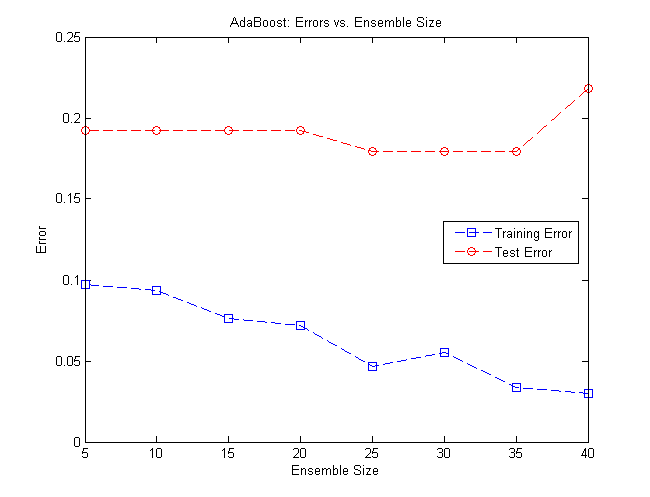
\includegraphics[width=1\linewidth]{img/boost_errors.png}
  \caption{AdaBoost}
  \label{fig:adaboost_errors}
 \end{subfigure}%
 \begin{subfigure}{.5\textwidth}
  \centering
  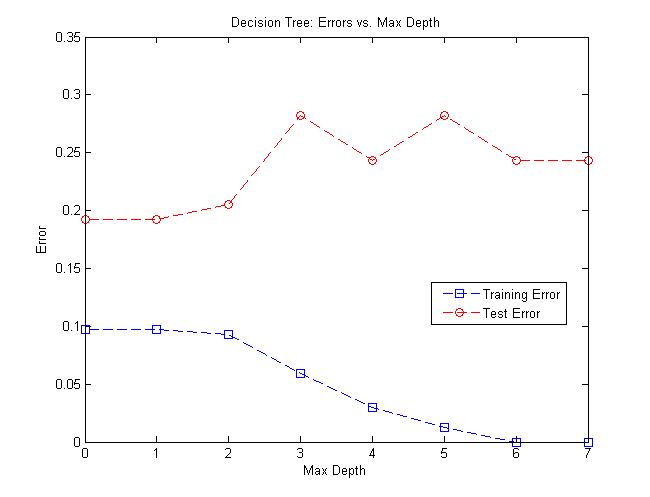
\includegraphics[width=1\linewidth]{img/tree_errors.png}
  \caption{Decision Tree}
  \label{fig:tree_errors}
 \end{subfigure}
\caption{Training and test errors for AdaBoost and decision tree. (a) AdaBoost training and test errors are a function of ensemble size. (b) Decision tree training and test errors are a function of maximum depth size.}
\label{fig:errors}
\end{figure}

Figure \ref{fig:adaboost_errors} presents the plot of training and test errors as a function of ensemble size. We see that the training error decreases reasonably. We also observe that the test error decreases until ensemble size 35. The test error at that point is a little under 20\%, which is reasonable.

Figure \ref{fig:tree_errors} presents the plot of training and test errors as a function of the maximum decision tree depth. We also see that the training error decreases reasonably. In fact it goes to zero at around a maximum depth of 6. At that point the test error is not good compared to smaller maximum depth sizes, which indicates that the decision tree is over-fitting the data. We also observe that the test error begins to increase early on. The best maximum depth is probably around 2. The test error is a little under 20\%, which is reasonable and comparable to the error from AdaBoost.

\section{Conclusion}
%\textbf{Summarize methodology and results.}

In this paper, we have motivated the problem of predicting the direction of the offensive play in a video. We have presented a framework for extracting useful features from a video and using them with machine learning to make predictions. Our results using boosting and decision trees yield promising accurate predictions.

%\section{Submission of papers to NIPS 2013}
%
%NIPS requires electronic submissions.  The electronic submission site is  
%\begin{center}
%   \url{http://papers.nips.cc}
%\end{center}
%
%Please read carefully the
%instructions below, and follow them faithfully.
%\subsection{Style}
%
%Papers to be submitted to NIPS 2013 must be prepared according to the
%instructions presented here. Papers may be only up to eight pages long,
%including figures. Since 2009 an additional ninth page \textit{containing only
%cited references} is allowed. Papers that exceed nine pages will not be
%reviewed, or in any other way considered for presentation at the conference.
%%This is a strict upper bound. 
%
%Please note that this year we have introduced automatic line number generation
%into the style file (for \LaTeXe and Word versions). This is to help reviewers
%refer to specific lines of the paper when they make their comments. Please do
%NOT refer to these line numbers in your paper as they will be removed from the
%style file for the final version of accepted papers.
%
%The margins in 2013 are the same as since 2007, which allow for $\approx 15\%$
%more words in the paper compared to earlier years. We are also again using 
%double-blind reviewing. Both of these require the use of new style files.
%
%Authors are required to use the NIPS \LaTeX{} style files obtainable at the
%NIPS website as indicated below. Please make sure you use the current files and
%not previous versions. Tweaking the style files may be grounds for rejection.
%
%%% \subsection{Double-blind reviewing}
%
%%% This year we are doing double-blind reviewing: the reviewers will not know 
%%% who the authors of the paper are. For submission, the NIPS style file will 
%%% automatically anonymize the author list at the beginning of the paper.
%
%%% Please write your paper in such a way to preserve anonymity. Refer to
%%% previous work by the author(s) in the third person, rather than first
%%% person. Do not provide Web links to supporting material at an identifiable
%%% web site.
%
%%%\subsection{Electronic submission}
%%%
%%% \textbf{THE SUBMISSION DEADLINE IS MAY 31st, 2013. SUBMISSIONS MUST BE LOGGED BY
%%% 23:00, MAY 31st, 2013, UNIVERSAL TIME}
%
%%% You must enter your submission in the electronic submission form available at
%%% the NIPS website listed above. You will be asked to enter paper title, name of
%%% all authors, keyword(s), and data about the contact
%%% author (name, full address, telephone, fax, and email). You will need to
%%% upload an electronic (postscript or pdf) version of your paper.
%
%%% You can upload more than one version of your paper, until the
%%% submission deadline. We strongly recommended uploading your paper in
%%% advance of the deadline, so you can avoid last-minute server congestion.
%%%
%%% Note that your submission is only valid if you get an e-mail
%%% confirmation from the server. If you do not get such an e-mail, please
%%% try uploading again. 
%
%
%\subsection{Retrieval of style files}
%
%The style files for NIPS and other conference information are available on the World Wide Web at
%\begin{center}
%   \url{http://www.nips.cc/}
%\end{center}
%The file \verb+nips2013.pdf+ contains these 
%instructions and illustrates the
%various formatting requirements your NIPS paper must satisfy. \LaTeX{}
%users can choose between two style files:
%\verb+nips11submit_09.sty+ (to be used with \LaTeX{} version 2.09) and
%\verb+nips11submit_e.sty+ (to be used with \LaTeX{}2e). The file
%\verb+nips2013.tex+ may be used as a ``shell'' for writing your paper. All you
%have to do is replace the author, title, abstract, and text of the paper with
%your own. The file
%\verb+nips2013.rtf+ is provided as a shell for MS Word users.
%
%The formatting instructions contained in these style files are summarized in
%sections \ref{gen_inst}, \ref{headings}, and \ref{others} below.
%
%%% \subsection{Keywords for paper submission}
%%% Your NIPS paper can be submitted with any of the following keywords (more than one keyword is possible for each paper):
%
%%% \begin{verbatim}
%%% Bioinformatics
%%% Biological Vision
%%% Brain Imaging and Brain Computer Interfacing
%%% Clustering
%%% Cognitive Science
%%% Control and Reinforcement Learning
%%% Dimensionality Reduction and Manifolds
%%% Feature Selection
%%% Gaussian Processes
%%% Graphical Models
%%% Hardware Technologies
%%% Kernels
%%% Learning Theory
%%% Machine Vision
%%% Margins and Boosting
%%% Neural Networks
%%% Neuroscience
%%% Other Algorithms and Architectures
%%% Other Applications
%%% Semi-supervised Learning
%%% Speech and Signal Processing
%%% Text and Language Applications
%
%%% \end{verbatim}
%
%\section{General formatting instructions}
%\label{gen_inst}
%
%The text must be confined within a rectangle 5.5~inches (33~picas) wide and
%9~inches (54~picas) long. The left margin is 1.5~inch (9~picas).
%Use 10~point type with a vertical spacing of 11~points. Times New Roman is the
%preferred typeface throughout. Paragraphs are separated by 1/2~line space,
%with no indentation.
%
%Paper title is 17~point, initial caps/lower case, bold, centered between
%2~horizontal rules. Top rule is 4~points thick and bottom rule is 1~point
%thick. Allow 1/4~inch space above and below title to rules. All pages should
%start at 1~inch (6~picas) from the top of the page.
%
%%The version of the paper submitted for review should have ``Anonymous Author(s)'' as the author of the paper.
%
%For the final version, authors' names are
%set in boldface, and each name is centered above the corresponding
%address. The lead author's name is to be listed first (left-most), and
%the co-authors' names (if different address) are set to follow. If
%there is only one co-author, list both author and co-author side by side.
%
%Please pay special attention to the instructions in section \ref{others}
%regarding figures, tables, acknowledgments, and references.
%
%\section{Headings: first level}
%\label{headings}
%
%First level headings are lower case (except for first word and proper nouns),
%flush left, bold and in point size 12. One line space before the first level
%heading and 1/2~line space after the first level heading.
%
%\subsection{Headings: second level}
%
%Second level headings are lower case (except for first word and proper nouns),
%flush left, bold and in point size 10. One line space before the second level
%heading and 1/2~line space after the second level heading.
%
%\subsubsection{Headings: third level}
%
%Third level headings are lower case (except for first word and proper nouns),
%flush left, bold and in point size 10. One line space before the third level
%heading and 1/2~line space after the third level heading.
%
%\section{Citations, figures, tables, references}
%\label{others}
%
%These instructions apply to everyone, regardless of the formatter being used.
%
%\subsection{Citations within the text}
%
%Citations within the text should be numbered consecutively. The corresponding
%number is to appear enclosed in square brackets, such as [1] or [2]-[5]. The
%corresponding references are to be listed in the same order at the end of the
%paper, in the \textbf{References} section. (Note: the standard
%\textsc{Bib\TeX} style \texttt{unsrt} produces this.) As to the format of the
%references themselves, any style is acceptable as long as it is used
%consistently.
%
%As submission is double blind, refer to your own published work in the 
%third person. That is, use ``In the previous work of Jones et al.\ [4]'',
%not ``In our previous work [4]''. If you cite your other papers that
%are not widely available (e.g.\ a journal paper under review), use
%anonymous author names in the citation, e.g.\ an author of the
%form ``A.\ Anonymous''. 
%
%
%\subsection{Footnotes}
%
%Indicate footnotes with a number\footnote{Sample of the first footnote} in the
%text. Place the footnotes at the bottom of the page on which they appear.
%Precede the footnote with a horizontal rule of 2~inches
%(12~picas).\footnote{Sample of the second footnote}
%
%\subsection{Figures}
%
%All artwork must be neat, clean, and legible. Lines should be dark
%enough for purposes of reproduction; art work should not be
%hand-drawn. The figure number and caption always appear after the
%figure. Place one line space before the figure caption, and one line
%space after the figure. The figure caption is lower case (except for
%first word and proper nouns); figures are numbered consecutively.
%
%Make sure the figure caption does not get separated from the figure.
%Leave sufficient space to avoid splitting the figure and figure caption.
%
%You may use color figures. 
%However, it is best for the
%figure captions and the paper body to make sense if the paper is printed
%either in black/white or in color.
%\begin{figure}[h]
%\begin{center}
%%\framebox[4.0in]{$\;$}
%\fbox{\rule[-.5cm]{0cm}{4cm} \rule[-.5cm]{4cm}{0cm}}
%\end{center}
%\caption{Sample figure caption.}
%\end{figure}
%
%\subsection{Tables}
%
%All tables must be centered, neat, clean and legible. Do not use hand-drawn
%tables. The table number and title always appear before the table. See
%Table~\ref{sample-table}.
%
%Place one line space before the table title, one line space after the table
%title, and one line space after the table. The table title must be lower case
%(except for first word and proper nouns); tables are numbered consecutively.
%
%\begin{table}[t]
%\caption{Sample table title}
%\label{sample-table}
%\begin{center}
%\begin{tabular}{ll}
%\multicolumn{1}{c}{\bf PART}  &\multicolumn{1}{c}{\bf DESCRIPTION}
%\\ \hline \\
%Dendrite         &Input terminal \\
%Axon             &Output terminal \\
%Soma             &Cell body (contains cell nucleus) \\
%\end{tabular}
%\end{center}
%\end{table}
%
%\section{Final instructions}
%Do not change any aspects of the formatting parameters in the style files.
%In particular, do not modify the width or length of the rectangle the text
%should fit into, and do not change font sizes (except perhaps in the
%\textbf{References} section; see below). Please note that pages should be
%numbered.
%
%\section{Preparing PostScript or PDF files}
%
%Please prepare PostScript or PDF files with paper size ``US Letter'', and
%not, for example, ``A4''. The -t
%letter option on dvips will produce US Letter files.
%
%Fonts were the main cause of problems in the past years. Your PDF file must
%only contain Type 1 or Embedded TrueType fonts. Here are a few instructions
%to achieve this.
%
%\begin{itemize}
%
%\item You can check which fonts a PDF files uses.  In Acrobat Reader,
%select the menu Files$>$Document Properties$>$Fonts and select Show All Fonts. You can
%also use the program \verb+pdffonts+ which comes with \verb+xpdf+ and is
%available out-of-the-box on most Linux machines.
%
%\item The IEEE has recommendations for generating PDF files whose fonts
%are also acceptable for NIPS. Please see
%\url{http://www.emfield.org/icuwb2010/downloads/IEEE-PDF-SpecV32.pdf}
%
%\item LaTeX users:
%
%\begin{itemize}
%
%\item Consider directly generating PDF files using \verb+pdflatex+
%(especially if you are a MiKTeX user). 
%PDF figures must be substituted for EPS figures, however.
%
%\item Otherwise, please generate your PostScript and PDF files with the following commands:
%\begin{verbatim} 
%dvips mypaper.dvi -t letter -Ppdf -G0 -o mypaper.ps
%ps2pdf mypaper.ps mypaper.pdf
%\end{verbatim}
%
%Check that the PDF files only contains Type 1 fonts. 
%%For the final version, please send us both the Postscript file and
%%the PDF file. 
%
%\item xfig "patterned" shapes are implemented with 
%bitmap fonts.  Use "solid" shapes instead. 
%\item The \verb+\bbold+ package almost always uses bitmap
%fonts.  You can try the equivalent AMS Fonts with command
%\begin{verbatim}
%\usepackage[psamsfonts]{amssymb}
%\end{verbatim}
% or use the following workaround for reals, natural and complex: 
%\begin{verbatim}
%\newcommand{\RR}{I\!\!R} %real numbers
%\newcommand{\Nat}{I\!\!N} %natural numbers 
%\newcommand{\CC}{I\!\!\!\!C} %complex numbers
%\end{verbatim}
%
%\item Sometimes the problematic fonts are used in figures
%included in LaTeX files. The ghostscript program \verb+eps2eps+ is the simplest
%way to clean such figures. For black and white figures, slightly better
%results can be achieved with program \verb+potrace+.
%\end{itemize}
%\item MSWord and Windows users (via PDF file):
%\begin{itemize}
%\item Install the Microsoft Save as PDF Office 2007 Add-in from
%\url{http://www.microsoft.com/downloads/details.aspx?displaylang=en\&familyid=4d951911-3e7e-4ae6-b059-a2e79ed87041}
%\item Select ``Save or Publish to PDF'' from the Office or File menu
%\end{itemize}
%\item MSWord and Mac OS X users (via PDF file):
%\begin{itemize}
%\item From the print menu, click the PDF drop-down box, and select ``Save
%as PDF...''
%\end{itemize}
%\item MSWord and Windows users (via PS file):
%\begin{itemize}
%\item To create a new printer
%on your computer, install the AdobePS printer driver and the Adobe Distiller PPD file from
%\url{http://www.adobe.com/support/downloads/detail.jsp?ftpID=204} {\it Note:} You must reboot your PC after installing the
%AdobePS driver for it to take effect.
%\item To produce the ps file, select ``Print'' from the MS app, choose
%the installed AdobePS printer, click on ``Properties'', click on ``Advanced.''
%\item Set ``TrueType Font'' to be ``Download as Softfont''
%\item Open the ``PostScript Options'' folder
%\item Select ``PostScript Output Option'' to be ``Optimize for Portability''
%\item Select ``TrueType Font Download Option'' to be ``Outline''
%\item Select ``Send PostScript Error Handler'' to be ``No''
%\item Click ``OK'' three times, print your file.
%\item Now, use Adobe Acrobat Distiller or ps2pdf to create a PDF file from
%the PS file. In Acrobat, check the option ``Embed all fonts'' if
%applicable.
%\end{itemize}
%
%\end{itemize}
%If your file contains Type 3 fonts or non embedded TrueType fonts, we will
%ask you to fix it. 
%
%\subsection{Margins in LaTeX}
% 
%Most of the margin problems come from figures positioned by hand using
%\verb+\special+ or other commands. We suggest using the command
%\verb+\includegraphics+
%from the graphicx package. Always specify the figure width as a multiple of
%the line width as in the example below using .eps graphics
%\begin{verbatim}
%   \usepackage[dvips]{graphicx} ... 
%   \includegraphics[width=0.8\linewidth]{myfile.eps} 
%\end{verbatim}
%or % Apr 2009 addition
%\begin{verbatim}
%   \usepackage[pdftex]{graphicx} ... 
%   \includegraphics[width=0.8\linewidth]{myfile.pdf} 
%\end{verbatim}
%for .pdf graphics. 
%See section 4.4 in the graphics bundle documentation (\url{http://www.ctan.org/tex-archive/macros/latex/required/graphics/grfguide.ps}) 
% 
%A number of width problems arise when LaTeX cannot properly hyphenate a
%line. Please give LaTeX hyphenation hints using the \verb+\-+ command.


\subsubsection*{Acknowledgments}

We would like to thank Dr. Alan Fern and  Dr. Sinisa Todorovic for motivating and formulating the problem of game play direction prediction by tracking wide receivers.

%Use unnumbered third level headings for the acknowledgments. All
%acknowledgments go at the end of the paper. Do not include 
%acknowledgments in the anonymized submission, only in the 
%final paper. 

\subsubsection*{References}

%References follow the acknowledgments. Use unnumbered third level heading for
%the references. Any choice of citation style is acceptable as long as you are
%consistent. It is permissible to reduce the font size to `small' (9-point) 
%when listing the references. {\bf Remember that this year you can use
%a ninth page as long as it contains \emph{only} cited references.}

\small{
[1] Bruce D. Lucas and Takeo Kanade. {\it An Iterative Image Registration Technique with an Application to Stereo Vision.} International Joint Conference on Artificial Intelligence, pages 674-679, 1981.

[2] Carlo Tomasi and Takeo Kanade. {\it Detection and Tracking of Point Features.} Carnegie Mellon University Technical Report CMU-CS-91-132, April 1991.

[3] Jianbo Shi and Carlo Tomasi. {\it Good Features to Track.} IEEE Conference on Computer Vision and Pattern Recognition, pages 593-600, 1994.

[4] Yoav Freund and Robert E Schapire. {\it A Decision-Theoretic Generalization of On-Line Learning and an Application to Boosting.} Proceedings of the Second European Conference on Computational Learning Theory, pages 23-37, 1995.

[5] J. Ross Quinlan. {\it Improved Use of Continuous Attributes in C4.5.} Journal of Artificial Intelligence Research, 4:77-90, 1996.
}

\end{document}
